\chapter{Analisi dei requisiti}
\label{chap:analisi-requisiti}

\section{Casi d'uso}
Per lo studio dei casi di utilizzo del prodotto sono stati creati dei diagrammi.
I diagrammi dei casi d'uso (in inglese \textit{Use Case Diagram}) sono diagrammi di tipo \gls{uml} dedicati alla descrizione delle funzioni o servizi offerti da un sistema, così come sono percepiti e utilizzati dagli attori che interagiscono col sistema stesso.
Essendo il progetto finalizzato alla creazione di un tool \gls{TermineSenzaAcronimo} per l'automazione di un processo, le interazioni da parte dell'utilizzatore devono essere ovviamente ridotte allo stretto necessario. Per questo motivo i diagrammi d'uso risultano semplici e in numero ridotto.

%--------------------------------------------------
% Casi d'uso obbligatori
%--------------------------------------------------

\begin{figure}[H]
    \vspace{2em}
    \centering
    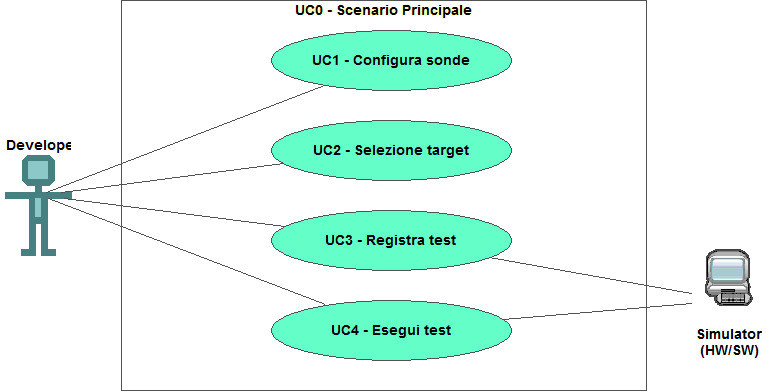
\includegraphics[alt={Testo alternativo dell'immagine}, width=0.75\columnwidth]{img/usecase/scenario-principale.jpeg}
    \caption{Use Case 0: Scenario principale}
    \label{fig:scenario_principale}
\end{figure}

\begin{usecase}{1}{Autenticazione Utente}
    \usecaseactors{Utente, Sistema}
    \usecasepre{L'utente si trova alla schermata di login.}
    \usecasedesc{Il Sistema verifica le credenziali inserite e, se corrette, crea una sessione autenticata protetta da \textit{token}.}
    \usecasepost{L'utente accede alle funzionalità permesse dal proprio ruolo.}
    \usecasealt{Se le credenziali non sono valide, viene mostrato un messaggio di errore.}
    \label{uc:uc1_auth}
\end{usecase}

\begin{usecase}{2}{Visualizzazione Dashboard Operativa}
    \usecaseactors{Operatore}
    \usecasepre{L'utente è autenticato e possiede il ruolo adeguato.}
    \usecasedesc{Il Sistema mostra in tempo reale code ai macchinari, \textit{lead time} e colli di bottiglia.}
    \usecasepost{I dati visualizzati sono sincronizzati con il database.}
    \usecasealt{Se i dati non sono disponibili, viene mostrato un avviso.}
    \label{uc:uc2_dashboard}
\end{usecase}

\begin{usecase}{3}{Drill-down Dettaglio Criticità}
    \usecaseactors{Operatore}
    \usecasepre{È selezionato un elemento critico nella dashboard.}
    \usecasedesc{Il Sistema fornisce grafici e log dettagliati relativi alla criticità selezionata.}
    \usecasepost{L'utente può decidere eventuali azioni correttive.}
    \usecasealt{Se i dati non sono disponibili, viene visualizzato un errore.}
    \label{uc:uc3_drilldown}
\end{usecase}

\begin{usecase}{4}{Analisi Dati Programmata}
    \usecaseactors{Scheduler}
    \usecasepre{È pianificato un \textit{job} di analisi con frequenza definita.}
    \usecasedesc{Il Scheduler avvia gli algoritmi di analisi senza intervento umano.}
    \usecasepost{I risultati sono memorizzati e resi disponibili alla dashboard.}
    \usecasealt{Se l’analisi fallisce, viene generato un log di errore.}
    \label{uc:uc4_analisi_programmata}
\end{usecase}

\begin{usecase}{5}{Rilevazione Anomalie e Colli di Bottiglia}
    \usecaseactors{Sistema}
    \usecasepre{Sono disponibili i dati di produzione aggiornati.}
    \usecasedesc{Algoritmi statistici individuano pattern critici nei tempi di coda e nei flussi di lavoro.}
    \usecasepost{Le anomalie rilevate sono contrassegnate come eventi critici.}
    \usecasealt{Se la qualità dei dati è insufficiente, l’analisi viene sospesa.}
    \label{uc:uc5_rilevazione_anomalie}
\end{usecase}

\begin{usecase}{6}{Generazione Suggerimenti da \gls{LLM}}
    \usecaseactors{Operatore, Servizio \textit{LLM}}
    \usecasepre{È stato selezionato almeno un evento critico.}
    \usecasedesc{Il Sistema invia i parametri dell’anomalia al \gls{LLM} e visualizza le azioni correttive suggerite.}
    \usecasepost{I suggerimenti sono archiviati e possono essere consultati in seguito.}
    \usecasealt{Se l'API restituisce un errore, viene mostrato un avviso.}
    \label{uc:uc6_llm_suggest}
\end{usecase}

\begin{usecase}{7}{Validazione e \textit{Data Cleaning} Automatico}
    \usecaseactors{Scheduler, Sistema}
    \usecasepre{È schedulato un job di validazione dati.}
    \usecasedesc{Il Sistema applica regole di integrità: valori mancanti, range ammessi, coerenza temporale; i record non conformi sono corretti o marcati come \textit{invalid}.}
    \usecasepost{Il dataset pulito è salvato, viene prodotto un report di esito.}
    \usecasealt{Se la percentuale di dati non validi supera la soglia, le analisi (UC4–UC5) vengono sospese e viene segnalato nei log.}
    \label{uc:uc7_data_cleaning}
\end{usecase}

%--------------------------------------------------
% Casi d'uso desiderabili
%--------------------------------------------------
\begin{usecase}{8}{Interazione Chatbot Gestionale}
    \usecaseactors{Utente}
    \usecasepre{L’utente è autenticato.}
    \usecasedesc{L’utente pone domande o impartisce comandi in linguaggio naturale; il Sistema risponde contestualmente.}
    \usecasepost{Le operazioni richieste vengono eseguite o i dati visualizzati.}
    \usecasealt{Se la richiesta non è compresa, viene chiesta una riformulazione.}
    \label{uc:uc8_chatbot}
\end{usecase}

\begin{usecase}{9}{Ricezione Notifiche Proattive}
    \usecaseactors{Utente, Sistema}
    \usecasepre{L’utente ha acconsentito a ricevere notifiche.}
    \usecasedesc{Al superamento di una soglia critica, il Sistema invia una notifica push.}
    \usecasepost{L’utente riceve l’avviso con il dettaglio dell’anomalia.}
    \usecasealt{Se il canale di consegna non è raggiungibile, il Sistema ritenta secondo un back-off esponenziale.}
    \label{uc:uc9_notifiche}
\end{usecase}

\begin{usecase}{10}{Accesso Versione Web}
    \usecaseactors{Utente}
    \usecasepre{Il browser supporta l'applicazione web.}
    \usecasedesc{L’utente accede alle stesse funzionalità della dashboard tramite interfaccia web responsiva.}
    \usecasepost{I dati e le azioni sono sincronizzati con l’app mobile.}
    \usecasealt{Se i dati non sono disponibili, viene visualizzato un errore.}
    \label{uc:uc10_web}
\end{usecase}

%--------------------------------------------------
% Casi d'uso facoltativi
%--------------------------------------------------
\begin{usecase}{11}{Sincronizzazione Offline}
    \usecaseactors{Operatore, Sistema}
    \usecasepre{Il dispositivo non ha connettività di rete.}
    \usecasedesc{L’Operatore continua ad utilizzare l’applicazione; tutte le operazioni vengono salvate in locale.}
    \usecasepost{Alla riconnessione, i dati locali vengono riallineati con il server.}
    \usecasealt{Se si verifica un conflitto con i dati salvati in locale, i cambiamenti vengono scartati.}
    \label{uc:uc11_offline}
\end{usecase}

%--------------------------------------------------
% Tracciamento dei requisiti
%--------------------------------------------------
\section{Tracciamento dei requisiti}
Il tracciamento mostra la copertura dei requisiti funzionali (F) classificati come
\textbf{N} (obbligatori), \textbf{D} (desiderabili) e \textbf{Z} (facoltativi).  
I requisiti qualitativi (Q) e di vincolo (V) restano invariati rispetto alla precedente analisi.

%--------------------------------------------------
% Tabella requisiti funzionali obbligatori
%--------------------------------------------------
\begin{center}
\rowcolors{1}{}{tableGray}
\begin{longtable}{|p{2.25cm}|p{7.75cm}|p{2.25cm}|}
\hline
\multicolumn{1}{|c|}{\textbf{Requisito}} & \multicolumn{1}{c|}{\textbf{Descrizione}} & \multicolumn{1}{c|}{\textbf{Use Case}}\\
\hline 
\endfirsthead
\rowcolor{white}
\multicolumn{3}{c}{{\bfseries \tablename\ \thetable{} -- Continuo}}\\
\hline
\multicolumn{1}{|c|}{\textbf{Requisito}} & \multicolumn{1}{c|}{\textbf{Descrizione}} & \multicolumn{1}{c|}{\textbf{Use Case}}\\
\hline 
\endhead
\hline
\rowcolor{white}
\multicolumn{3}{|r|}{{Continua nella prossima pagina...}}\\
\hline
\endfoot
\endlastfoot
O01 & Il sistema consente l'autenticazione sicura dell'utente & UC1 \\ \hline
O02 & Visualizzare in tempo reale le metriche di produzione & UC2 \\ \hline
O03 & Consentire l’analisi dettagliata di una criticità & UC3 \\ \hline
O04 & Eseguire analisi dati in modalità programmata & UC4 \\ \hline
O05 & Rilevare automaticamente anomalie e colli di bottiglia & UC5 \\ \hline
O06 & Fornire suggerimenti tramite servizio \textit{LLM} & UC6 \\ \hline
O07 & Validare e ripulire i dati prima dell’analisi & UC7 \\ \hline
\caption{Tracciamento requisiti funzionali obbligatori (RFN).}
\label{tab:requisiti_fun_obbl}
\end{longtable}
\end{center}

%--------------------------------------------------
% Tabella requisiti funzionali desiderabili
%--------------------------------------------------
\begin{center}
\rowcolors{1}{}{tableGray}
\begin{longtable}{|p{2.25cm}|p{7.75cm}|p{2.25cm}|}
\hline
\multicolumn{1}{|c|}{\textbf{Requisito}} & \multicolumn{1}{c|}{\textbf{Descrizione}} & \multicolumn{1}{c|}{\textbf{Use Case}}\\
\hline 
\endfirsthead
\rowcolor{white}
\multicolumn{3}{c}{{\bfseries \tablename\ \thetable{} -- Continuo}}\\
\hline
\multicolumn{1}{|c|}{\textbf{Requisito}} & \multicolumn{1}{c|}{\textbf{Descrizione}} & \multicolumn{1}{c|}{\textbf{Use Case}}\\
\hline 
\endhead
\hline
\rowcolor{white}
\multicolumn{3}{|r|}{{Continua nella prossima pagina...}}\\
\hline
\endfoot
\endlastfoot
D01 & Interagire con il sistema tramite chatbot & UC8 \\ \hline
D02 & Ricevere notifiche push o \textit{e-mail} al superamento di soglie & UC9 \\ \hline
D03 & Accedere alla dashboard da interfaccia web responsiva & UC10 \\ \hline
\caption{Tracciamento requisiti funzionali desiderabili (RFD).}
\label{tab:requisiti_fun_des}
\end{longtable}
\end{center}

%--------------------------------------------------
% Tabella requisiti funzionali facoltativi
%--------------------------------------------------
\begin{center}
\rowcolors{1}{}{tableGray}
\begin{longtable}{|p{2.25cm}|p{7.75cm}|p{2.25cm}|}
\hline
\multicolumn{1}{|c|}{\textbf{Requisito}} & \multicolumn{1}{c|}{\textbf{Descrizione}} & \multicolumn{1}{c|}{\textbf{Use Case}}\\
\hline 
\endfirsthead
\rowcolor{white}
\multicolumn{3}{c}{{\bfseries \tablename\ \thetable{} -- Continuo}}\\
\hline
\multicolumn{1}{|c|}{\textbf{Requisito}} & \multicolumn{1}{c|}{\textbf{Descrizione}} & \multicolumn{1}{c|}{\textbf{Use Case}}\\
\hline 
\endhead
\hline
\rowcolor{white}
\multicolumn{3}{|r|}{{Continua nella prossima pagina...}}\\
\hline
\endfoot
\endlastfoot
F01 & Garantire la continuità operativa in assenza di connessione & UC11 \\ \hline
\caption{Tracciamento requisiti funzionali facoltativi (RFZ).}
\label{tab:requisiti_fun_fac}
\end{longtable}
\end{center}
